\documentclass{report}
\usepackage{fancyhdr} % Required for custom headers
\usepackage{lastpage} % Required to determine the last page for the footer
\usepackage{extramarks} % Required for headers and footers
\usepackage{graphicx} % Required to insert images

\usepackage{amsmath}
\usepackage{graphicx} 
\usepackage{float}
%\usepackage{amsfont}
%\usepackage{amssymb}

\usepackage{multicol}
% Margins
\topmargin=-0.5in
\evensidemargin=0in
\oddsidemargin=-0.5in
\textwidth=7.5in
\textheight=9.0in
\headsep=0.25in 


\pagestyle{fancy}

%\rhead{\textbf{Marshall's Recipes}} % Top right header
%\lhead{\textbf{Curry Stir Fry}}
%\chead{ }
%\title{Curry Stir Fry}

\begin{document}
%\vspace{8mm}
%\textbf{PRELIMINARIES:}


\bigskip

\bigskip

\begin{multicols}{2}
\textbf{Ingredients}
\begin{itemize}
\item 1 lb baby bella muhsrooms \newline (130 kCal / 13 gP / 0 gF / 13 gC)
\item 2 cups jasmine rice \quad (1280 kCal / 24 gP / 0 gF / 288 gC)
\item 1.5 lbs brussels sprouts (360 kCal/ 24 gP/ 0 gF/ 64 gC)
\item 2 tbsp. olive oil (for brussels sprouts) \newline (238 kCal / 0 gP / 28 gF / 0 gC)
\item 4 tbsp. butter \quad (408 kCal / 0 gP / 48 gF / 0 gC)
\item 3 cups vegetable or chicken broth
\item 6 cloves of garlic
\item 2 tsp. balsamic vinegar
\item $\frac{1}{4}$ tsp. salt
\item $\frac{1}{2}$ tsp. dried thyme
\item $\frac{1}{2}$ tsp. cayenne pepper



\end{itemize}


\columnbreak
\textbf{Procedure:}
\medskip


\begin{enumerate}

\item Slice the mushrooms and mince the garlic.
\item Add the mushrooms, garlic, thyme, pepper, salt, and 1 Tbsp butter to a deep skillet. Sauté over medium heat until the mushrooms have released all of their water and the water has evaporated off the bottom of the skillet. Cut the rough stems from the bottom of the brussels sprouts and add to steamer basket in a pot with enough water to just barely come above the bottom of the steamer basket. Place on high heat with a lid. 
\item Rinse and drain the rice. Add rice and 3 tbsp. butter to mushrooms and continue to sauté for about two minutes more. 
\item Add the vegetable broth to the skillet and stir to dissolve any browned bits off the bottom of the skillet. 
\item Place a lid on the skillet, turn the heat up to medium-high, and allow the broth to come up to a full boil. When it reaches a full boil, turn the heat down to low, or just above low, so the broth remains simmering. 

\item Let the rice simmer for 15 minutes without stirring or removing the lid. After 15 minutes, remove the pan from the heat and let the rice rest for another 5 minutes, without removing the lid. Once the brussels sprouts are done, remove from steamer and place into a large bowl. Add 2 tbsp. olive oil and seasonings (I use red pepper flakes, garlic powder, and salt) and stir to coat evenly. 
\item Finally, remove the lid and fluff the rice with a fork. Stir in balsamic vinegar. Taste and add salt or pepper, if desired. Top with chopped fresh parsley as a garnish.

\begin{table}[H]
  \begin{center}
    \caption{Macro totals}
    \label{tab:table1}
    \begin{tabular}{c|c|c|c} % <-- Alignments: 1st column left, 2nd middle and 3rd right, with vertical lines in between
      \textbf{Calories} & \textbf{Protein} & \textbf{Fat} & \textbf{Carbs}\\
      \hline
      2416 kCal & 61 g & 76 g & 365 g\\
    \end{tabular}
  \end{center}
\end{table}
 
\end{enumerate}
\end{multicols}




%\begin{center}
%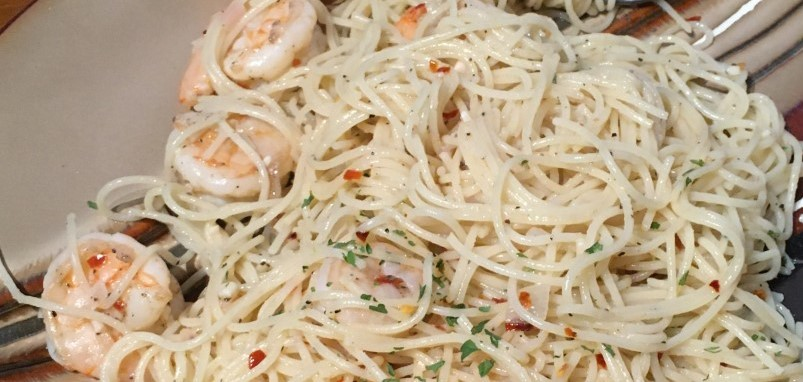
\includegraphics[scale=0.65]{Pasta/Shrimp Scampi/Shrimp Scampi.jpg}
%\end{center}


\end{document}